% Created by tikzDevice version 0.10.1 on 2016-05-09 14:41:45
% !TEX encoding = UTF-8 Unicode
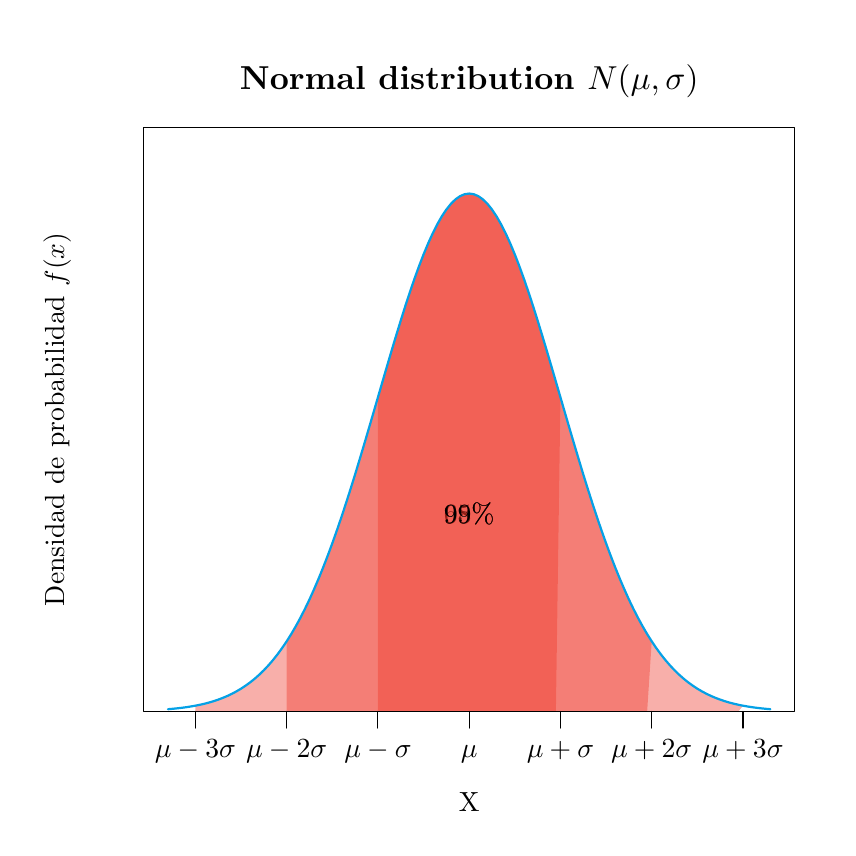
\begin{tikzpicture}[x=1pt,y=1pt]
\definecolor{fillColor}{RGB}{255,255,255}
\path[use as bounding box,fill=fillColor,fill opacity=0.00] (0,0) rectangle (289.08,289.08);
\begin{scope}
\path[clip] (  0.00,  0.00) rectangle (289.08,289.08);
\definecolor{drawColor}{RGB}{0,0,0}

\node[text=drawColor,anchor=base,inner sep=0pt, outer sep=0pt, scale=  1.20] at (159.54,266.89) {\bfseries Normal distribution $N(\mu,\sigma)$};

\node[text=drawColor,anchor=base,inner sep=0pt, outer sep=0pt, scale=  1.00] at (159.54,  6.00) {X};

\node[text=drawColor,rotate= 90.00,anchor=base,inner sep=0pt, outer sep=0pt, scale=  1.00] at ( 13.20,147.54) {Densidad de probabilidad $f(x)$};
\end{scope}
\begin{scope}
\path[clip] (  0.00,  0.00) rectangle (289.08,289.08);
\definecolor{drawColor}{RGB}{0,0,0}

\path[draw=drawColor,line width= 0.4pt,line join=round,line cap=round] (159.54, 42.00) -- (159.54, 42.00);

\path[draw=drawColor,line width= 0.4pt,line join=round,line cap=round] (159.54, 42.00) -- (159.54, 36.00);

\node[text=drawColor,anchor=base,inner sep=0pt, outer sep=0pt, scale=  1.00] at (159.54, 25.20) {$\mu$};

\path[draw=drawColor,line width= 0.4pt,line join=round,line cap=round] (126.56, 42.00) -- (192.52, 42.00);

\onslide<2>{\path[draw=drawColor,line width= 0.4pt,line join=round,line cap=round] (126.56, 42.00) -- (126.56, 36.00);

\path[draw=drawColor,line width= 0.4pt,line join=round,line cap=round] (192.52, 42.00) -- (192.52, 36.00);

\node[text=drawColor,anchor=base,inner sep=0pt, outer sep=0pt, scale=  1.00] at (126.56, 25.20) {$\mu-\sigma$};

\node[text=drawColor,anchor=base,inner sep=0pt, outer sep=0pt, scale=  1.00] at (192.52, 25.20) {$\mu+\sigma$};
}
\end{scope}

\onslide<2>{
\begin{scope}
\path[clip] ( 42.00, 42.00) rectangle (277.08,253.08);
\definecolor{fillColor}{RGB}{238,50,36}

\path[fill=fillColor,fill opacity=0.39] (126.56, 42.00) --
	(126.56,155.50) --
	(128.21,161.17) --
	(129.86,166.81) --
	(131.51,172.39) --
	(133.16,177.88) --
	(134.81,183.25) --
	(136.45,188.47) --
	(138.10,193.50) --
	(139.75,198.30) --
	(141.40,202.86) --
	(143.05,207.14) --
	(144.70,211.11) --
	(146.35,214.74) --
	(148.00,218.01) --
	(149.65,220.90) --
	(151.30,223.37) --
	(152.94,225.43) --
	(154.59,227.04) --
	(156.24,228.20) --
	(157.89,228.90) --
	(159.54,229.13) --
	(161.19,228.90) --
	(162.84,228.20) --
	(164.49,227.04) --
	(166.14,225.43) --
	(167.78,223.37) --
	(169.43,220.90) --
	(171.08,218.01) --
	(172.73,214.74) --
	(174.38,211.11) --
	(176.03,207.14) --
	(177.68,202.86) --
	(179.33,198.30) --
	(180.98,193.50) --
	(182.63,188.47) --
	(184.27,183.25) --
	(185.92,177.88) --
	(187.57,172.39) --
	(189.22,166.81) --
	(190.87,161.17) --
	(192.52,155.50) --
	(190.87, 42.00) --
	cycle;
\definecolor{drawColor}{RGB}{0,0,0}

\node[text=drawColor,anchor=base,inner sep=0pt, outer sep=0pt, scale=  1.00] at (159.54,109.86) {$68\%$};
\end{scope}
}
\onslide<3>{
\begin{scope}
\path[clip] (  0.00,  0.00) rectangle (289.08,289.08);
\definecolor{drawColor}{RGB}{0,0,0}

\path[draw=drawColor,line width= 0.4pt,line join=round,line cap=round] ( 93.58, 42.00) -- (225.50, 42.00);

\path[draw=drawColor,line width= 0.4pt,line join=round,line cap=round] ( 93.58, 42.00) -- ( 93.58, 36.00);

\path[draw=drawColor,line width= 0.4pt,line join=round,line cap=round] (225.50, 42.00) -- (225.50, 36.00);

\node[text=drawColor,anchor=base,inner sep=0pt, outer sep=0pt, scale=  1.00] at ( 93.58, 25.20) {$\mu-2\sigma$};

\node[text=drawColor,anchor=base,inner sep=0pt, outer sep=0pt, scale=  1.00] at (225.50, 25.20) {$\mu+2\sigma$};
\end{scope}
\begin{scope}
\path[clip] ( 42.00, 42.00) rectangle (277.08,253.08);
\definecolor{fillColor}{RGB}{238,50,36}

\path[fill=fillColor,fill opacity=0.39] ( 93.58, 42.00) --
	( 93.58, 67.33) --
	( 95.23, 69.95) --
	( 96.88, 72.78) --
	( 98.53, 75.80) --
	(100.18, 79.03) --
	(101.83, 82.47) --
	(103.47, 86.12) --
	(105.12, 89.97) --
	(106.77, 94.03) --
	(108.42, 98.29) --
	(110.07,102.75) --
	(111.72,107.40) --
	(113.37,112.23) --
	(115.02,117.23) --
	(116.67,122.38) --
	(118.32,127.67) --
	(119.96,133.09) --
	(121.61,138.60) --
	(123.26,144.19) --
	(124.91,149.83) --
	(126.56,155.50) --
	(128.21,161.17) --
	(129.86,166.81) --
	(131.51,172.39) --
	(133.16,177.88) --
	(134.81,183.25) --
	(136.45,188.47) --
	(138.10,193.50) --
	(139.75,198.30) --
	(141.40,202.86) --
	(143.05,207.14) --
	(144.70,211.11) --
	(146.35,214.74) --
	(148.00,218.01) --
	(149.65,220.90) --
	(151.30,223.37) --
	(152.94,225.43) --
	(154.59,227.04) --
	(156.24,228.20) --
	(157.89,228.90) --
	(159.54,229.13) --
	(161.19,228.90) --
	(162.84,228.20) --
	(164.49,227.04) --
	(166.14,225.43) --
	(167.78,223.37) --
	(169.43,220.90) --
	(171.08,218.01) --
	(172.73,214.74) --
	(174.38,211.11) --
	(176.03,207.14) --
	(177.68,202.86) --
	(179.33,198.30) --
	(180.98,193.50) --
	(182.63,188.47) --
	(184.27,183.25) --
	(185.92,177.88) --
	(187.57,172.39) --
	(189.22,166.81) --
	(190.87,161.17) --
	(192.52,155.50) --
	(194.17,149.83) --
	(195.82,144.19) --
	(197.47,138.60) --
	(199.12,133.09) --
	(200.76,127.67) --
	(202.41,122.38) --
	(204.06,117.23) --
	(205.71,112.23) --
	(207.36,107.40) --
	(209.01,102.75) --
	(210.66, 98.29) --
	(212.31, 94.03) --
	(213.96, 89.97) --
	(215.61, 86.12) --
	(217.25, 82.47) --
	(218.90, 79.03) --
	(220.55, 75.80) --
	(222.20, 72.78) --
	(223.85, 69.95) --
	(225.50, 67.33) --
	(223.85, 42.00) --
	cycle;
\definecolor{drawColor}{RGB}{0,0,0}

\node[text=drawColor,anchor=base,inner sep=0pt, outer sep=0pt, scale=  1.00] at (159.54,109.86) {$95\%$};
\end{scope}
}

\onslide<4>{
\begin{scope}
\path[clip] (  0.00,  0.00) rectangle (289.08,289.08);
\definecolor{drawColor}{RGB}{0,0,0}

\path[draw=drawColor,line width= 0.4pt,line join=round,line cap=round] ( 60.60, 42.00) -- (258.48, 42.00);

\path[draw=drawColor,line width= 0.4pt,line join=round,line cap=round] ( 60.60, 42.00) -- ( 60.60, 36.00);

\path[draw=drawColor,line width= 0.4pt,line join=round,line cap=round] (258.48, 42.00) -- (258.48, 36.00);

\node[text=drawColor,anchor=base,inner sep=0pt, outer sep=0pt, scale=  1.00] at ( 60.60, 25.20) {$\mu-3\sigma$};

\node[text=drawColor,anchor=base,inner sep=0pt, outer sep=0pt, scale=  1.00] at (258.48, 25.20) {$\mu+3\sigma$};
\end{scope}
}

\begin{scope}
\path[clip] ( 42.00, 42.00) rectangle (277.08,253.08);
\definecolor{fillColor}{RGB}{238,50,36}
\onslide<4>{
\path[fill=fillColor,fill opacity=0.39] ( 60.60, 42.00) --
	( 60.60, 44.08) --
	( 62.25, 44.41) --
	( 63.90, 44.79) --
	( 65.55, 45.22) --
	( 67.20, 45.71) --
	( 68.85, 46.27) --
	( 70.49, 46.89) --
	( 72.14, 47.59) --
	( 73.79, 48.37) --
	( 75.44, 49.25) --
	( 77.09, 50.22) --
	( 78.74, 51.31) --
	( 80.39, 52.50) --
	( 82.04, 53.83) --
	( 83.69, 55.29) --
	( 85.34, 56.89) --
	( 86.98, 58.64) --
	( 88.63, 60.55) --
	( 90.28, 62.63) --
	( 91.93, 64.89) --
	( 93.58, 67.33) --
	( 95.23, 69.95) --
	( 96.88, 72.78) --
	( 98.53, 75.80) --
	(100.18, 79.03) --
	(101.83, 82.47) --
	(103.47, 86.12) --
	(105.12, 89.97) --
	(106.77, 94.03) --
	(108.42, 98.29) --
	(110.07,102.75) --
	(111.72,107.40) --
	(113.37,112.23) --
	(115.02,117.23) --
	(116.67,122.38) --
	(118.32,127.67) --
	(119.96,133.09) --
	(121.61,138.60) --
	(123.26,144.19) --
	(124.91,149.83) --
	(126.56,155.50) --
	(128.21,161.17) --
	(129.86,166.81) --
	(131.51,172.39) --
	(133.16,177.88) --
	(134.81,183.25) --
	(136.45,188.47) --
	(138.10,193.50) --
	(139.75,198.30) --
	(141.40,202.86) --
	(143.05,207.14) --
	(144.70,211.11) --
	(146.35,214.74) --
	(148.00,218.01) --
	(149.65,220.90) --
	(151.30,223.37) --
	(152.94,225.43) --
	(154.59,227.04) --
	(156.24,228.20) --
	(157.89,228.90) --
	(159.54,229.13) --
	(161.19,228.90) --
	(162.84,228.20) --
	(164.49,227.04) --
	(166.14,225.43) --
	(167.78,223.37) --
	(169.43,220.90) --
	(171.08,218.01) --
	(172.73,214.74) --
	(174.38,211.11) --
	(176.03,207.14) --
	(177.68,202.86) --
	(179.33,198.30) --
	(180.98,193.50) --
	(182.63,188.47) --
	(184.27,183.25) --
	(185.92,177.88) --
	(187.57,172.39) --
	(189.22,166.81) --
	(190.87,161.17) --
	(192.52,155.50) --
	(194.17,149.83) --
	(195.82,144.19) --
	(197.47,138.60) --
	(199.12,133.09) --
	(200.76,127.67) --
	(202.41,122.38) --
	(204.06,117.23) --
	(205.71,112.23) --
	(207.36,107.40) --
	(209.01,102.75) --
	(210.66, 98.29) --
	(212.31, 94.03) --
	(213.96, 89.97) --
	(215.61, 86.12) --
	(217.25, 82.47) --
	(218.90, 79.03) --
	(220.55, 75.80) --
	(222.20, 72.78) --
	(223.85, 69.95) --
	(225.50, 67.33) --
	(227.15, 64.89) --
	(228.80, 62.63) --
	(230.45, 60.55) --
	(232.10, 58.64) --
	(233.74, 56.89) --
	(235.39, 55.29) --
	(237.04, 53.83) --
	(238.69, 52.50) --
	(240.34, 51.31) --
	(241.99, 50.22) --
	(243.64, 49.25) --
	(245.29, 48.37) --
	(246.94, 47.59) --
	(248.59, 46.89) --
	(250.23, 46.27) --
	(251.88, 45.71) --
	(253.53, 45.22) --
	(255.18, 44.79) --
	(256.83, 44.41) --
	(258.48, 44.08) --
	(256.83, 42.00) --
	cycle;
\definecolor{drawColor}{RGB}{0,0,0}

\node[text=drawColor,anchor=base,inner sep=0pt, outer sep=0pt, scale=  1.00] at (159.54,109.86) {$99\%$};
}

\definecolor{drawColor}{RGB}{5,161,230}

\path[draw=drawColor,line width= 0.8pt,line join=round,line cap=round] ( 50.71, 42.81) --
	( 52.36, 42.95) --
	( 54.00, 43.12) --
	( 55.65, 43.31) --
	( 57.30, 43.53) --
	( 58.95, 43.79) --
	( 60.60, 44.08) --
	( 62.25, 44.41) --
	( 63.90, 44.79) --
	( 65.55, 45.22) --
	( 67.20, 45.71) --
	( 68.85, 46.27) --
	( 70.49, 46.89) --
	( 72.14, 47.59) --
	( 73.79, 48.37) --
	( 75.44, 49.25) --
	( 77.09, 50.22) --
	( 78.74, 51.31) --
	( 80.39, 52.50) --
	( 82.04, 53.83) --
	( 83.69, 55.29) --
	( 85.34, 56.89) --
	( 86.98, 58.64) --
	( 88.63, 60.55) --
	( 90.28, 62.63) --
	( 91.93, 64.89) --
	( 93.58, 67.33) --
	( 95.23, 69.95) --
	( 96.88, 72.78) --
	( 98.53, 75.80) --
	(100.18, 79.03) --
	(101.83, 82.47) --
	(103.47, 86.12) --
	(105.12, 89.97) --
	(106.77, 94.03) --
	(108.42, 98.29) --
	(110.07,102.75) --
	(111.72,107.40) --
	(113.37,112.23) --
	(115.02,117.23) --
	(116.67,122.38) --
	(118.32,127.67) --
	(119.96,133.09) --
	(121.61,138.60) --
	(123.26,144.19) --
	(124.91,149.83) --
	(126.56,155.50) --
	(128.21,161.17) --
	(129.86,166.81) --
	(131.51,172.39) --
	(133.16,177.88) --
	(134.81,183.25) --
	(136.45,188.47) --
	(138.10,193.50) --
	(139.75,198.30) --
	(141.40,202.86) --
	(143.05,207.14) --
	(144.70,211.11) --
	(146.35,214.74) --
	(148.00,218.01) --
	(149.65,220.90) --
	(151.30,223.37) --
	(152.94,225.43) --
	(154.59,227.04) --
	(156.24,228.20) --
	(157.89,228.90) --
	(159.54,229.13) --
	(161.19,228.90) --
	(162.84,228.20) --
	(164.49,227.04) --
	(166.14,225.43) --
	(167.78,223.37) --
	(169.43,220.90) --
	(171.08,218.01) --
	(172.73,214.74) --
	(174.38,211.11) --
	(176.03,207.14) --
	(177.68,202.86) --
	(179.33,198.30) --
	(180.98,193.50) --
	(182.63,188.47) --
	(184.27,183.25) --
	(185.92,177.88) --
	(187.57,172.39) --
	(189.22,166.81) --
	(190.87,161.17) --
	(192.52,155.50) --
	(194.17,149.83) --
	(195.82,144.19) --
	(197.47,138.60) --
	(199.12,133.09) --
	(200.76,127.67) --
	(202.41,122.38) --
	(204.06,117.23) --
	(205.71,112.23) --
	(207.36,107.40) --
	(209.01,102.75) --
	(210.66, 98.29) --
	(212.31, 94.03) --
	(213.96, 89.97) --
	(215.61, 86.12) --
	(217.25, 82.47) --
	(218.90, 79.03) --
	(220.55, 75.80) --
	(222.20, 72.78) --
	(223.85, 69.95) --
	(225.50, 67.33) --
	(227.15, 64.89) --
	(228.80, 62.63) --
	(230.45, 60.55) --
	(232.10, 58.64) --
	(233.74, 56.89) --
	(235.39, 55.29) --
	(237.04, 53.83) --
	(238.69, 52.50) --
	(240.34, 51.31) --
	(241.99, 50.22) --
	(243.64, 49.25) --
	(245.29, 48.37) --
	(246.94, 47.59) --
	(248.59, 46.89) --
	(250.23, 46.27) --
	(251.88, 45.71) --
	(253.53, 45.22) --
	(255.18, 44.79) --
	(256.83, 44.41) --
	(258.48, 44.08) --
	(260.13, 43.79) --
	(261.78, 43.53) --
	(263.43, 43.31) --
	(265.08, 43.12) --
	(266.72, 42.95) --
	(268.37, 42.81);
\end{scope}
\begin{scope}
\path[clip] (  0.00,  0.00) rectangle (289.08,289.08);
\definecolor{drawColor}{RGB}{0,0,0}

\path[draw=drawColor,line width= 0.4pt,line join=round,line cap=round] ( 42.00, 42.00) --
	(277.08, 42.00) --
	(277.08,253.08) --
	( 42.00,253.08) --
	( 42.00, 42.00);
\end{scope}
\end{tikzpicture}
